\section{Wdrożenie i testy}
Po wdrożeniu aplikacja została przetestowana pod względem funkcjonalnym. Testy wypadły pozytywnie.

\begin{figure}[H]
	\centering
	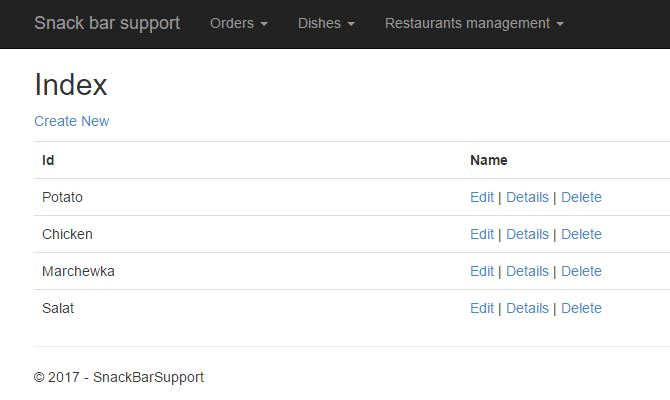
\includegraphics[width=\textwidth]{ingredients}
	\caption{Przykład listy - \textit{Ingredients}}
	\label{rys:ingredients}
\end{figure}

\begin{figure}[H]
\centering
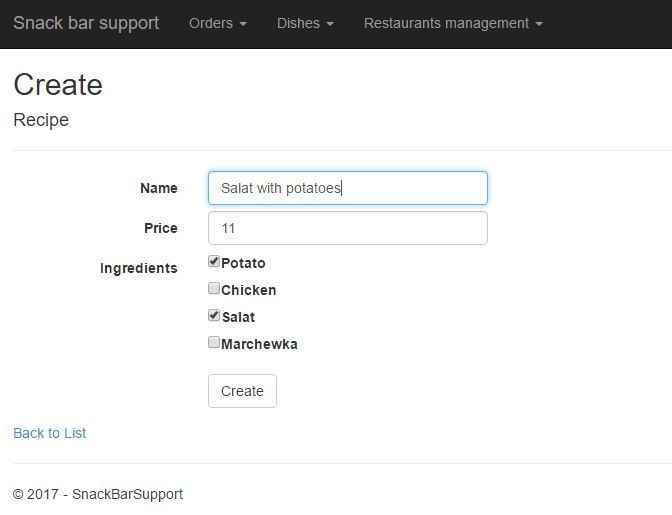
\includegraphics[width=\textwidth]{createRecipe}
\caption{Tworzenie nowego przepisu}
\label{rys:createRecipe}
\end{figure}

\begin{figure}[H]
\centering
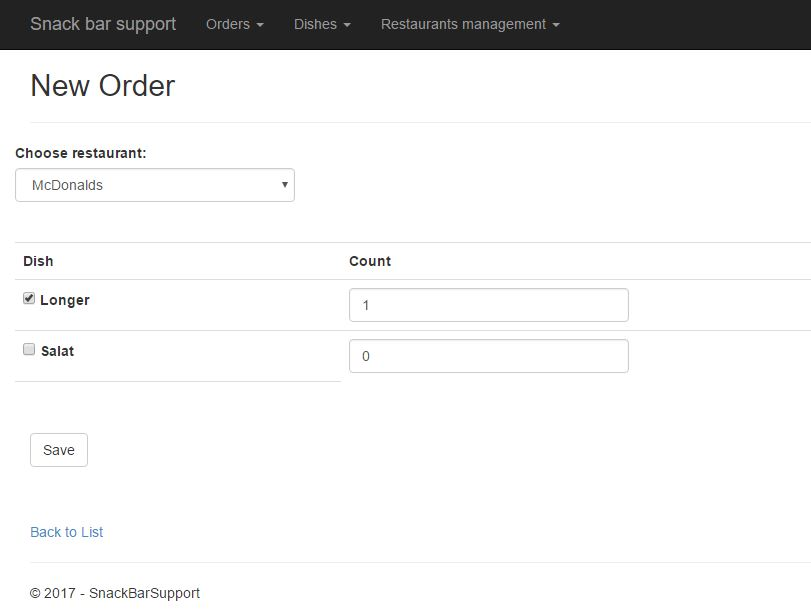
\includegraphics[width=\textwidth]{newOrder}
\caption{Dodawanie nowego zamówienia}
\label{rys:newOrder}
\end{figure}

\begin{figure}[H]
\centering
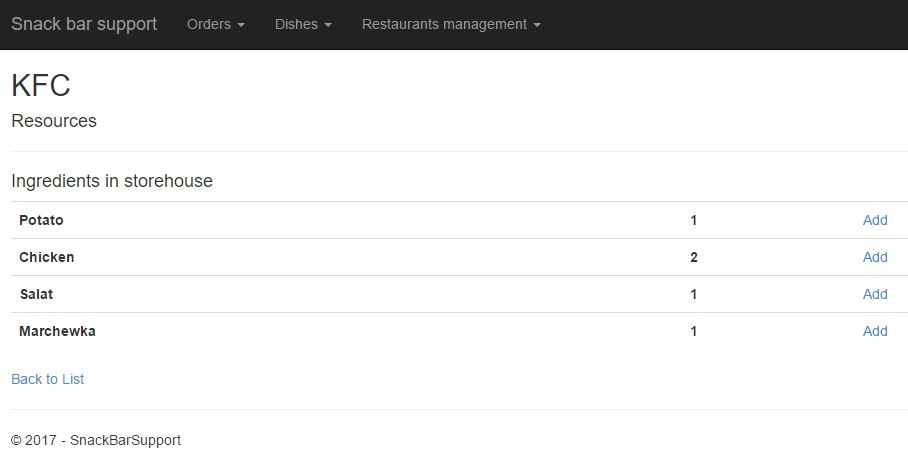
\includegraphics[width=\textwidth]{resources}
\caption{Uzupełnianie zasobów}
\label{rys:resources}
\end{figure}

\subsection{Replikacja}
Replikacja pomiędzy węzłami na podstawie replikacji dziennika logów daje gwarancję przeniesienia wszystkich operacji wykonanych na węźle \textit{Primary}. W czasie testów aplikacji, jak również podczas bezpośredniego obciążania bazy danych dużą ilością operacji zapisu i modyfikacji danych nie zauważono problemów z niepełną lub błędną replikacją. \\
Głównym problemem związanym z replikacją w systemie MongoDB jest możliwy \textit{replication lag}, a więc długość okresu w którym dane na poszczególnych węzłach różnią się. \\
W przypadku ustawień domyślnych aplikacji klienckich nie ma on znaczenia - aplikacje te czytają i zapisują tylko z węzła \textit{Primary}. W celu zwiększenia skalowalności systemu, zdecydowano jednak na zmianę tych ustawień i wymuszenie odczytu z pozostałych węzłów. W tym wypadku opóźnienie replikacji na poziomie kilkudziesięciu czy kilkuset milisekund może spowodować odczyt nieaktualnych danych, co też udało się zaobserwować przy operacjach typu \textit{edytuj dane} i \textit{pobierz nową wartość}. W celu zminimalizowania ryzyka wystąpienia takiej sytuacji, skorzystano z funkcjonalności \textit{Write Concern} MongoDB - każdy zapis w bazie danych musi zostać wykonany na minimum \textit{n} instancjach zanim system poinformuje aplikację kliencką o sukciesie operacji. Ustawienie wartości \textit{n} na 2 w przypadku 3-elementowego zestawu replik jest najlepszym kompromisem. Z jednej strony gwarantuje zapis do minimum jedego z węzłów \textit{Secondary} przed poinformowaniem aplikacji serwerowej o sukciesie zapisu, z drugiej strony nie wpływa negatywnie na aplikację w przypadku awarii jednego z węzłów - ustawienie \textit{Write Concern} na 3 przy 2 dostępnych węzłach powoduje \textit{timeout} interfejsu webowego przy każdej operacji zapisu.

\subsection{Odpornośc na awarie}
W celu zapewnienia wysokiej dostępności mechanizm \textit{failover} powienin być możliwie "przeźroczysty" dla użytkownika, tj. użytkownk nie powinien zauważać przestoju w działaniu usługi, przerwania sesji, ograniczenia funkcjonalności aplikacji. Mechanizm MongoDB oferuje te możliwości w przypadku zestawu replik składającego się z 3 węzłów przy awarii 1 węzła. \\
Przeprowadzone testy wykazały, że mechanizm \textit{failover} w praktyce trwa kilka do kilkunastu sekund. W najgorszym scenariuszu, tj. użytkownik wykonuje żądanie zapisu tuż po awarii węzła \textit{Primary}, użytkownik zostanie poinformowany o błędzie, przy próbie ponowienia żądania wybory nowego węzła \textit{Primary} już się odbyły i żądanie może zostać skutecznie obsłużone. Awarie węzłów \textit{seconary}, lub próba odczytu danych po awarii węzła objawiają się dłuższym wykonywaniem pierwszego żądania po awarii - aplikacja kliencka odkrywa aktualną konfigurację zestawu replik i wybiera dostępne węzły do tego i przyszłych żądań. Następne żądania wykonywane są już z normalną wydajnością, co oznacza, iż użytkownik końcowy nie jest świadom zaistniałej awarii. Można to uzyskać poprzez ustawienie pozwalające czytać aplikacji klienckiej dane z węzłów \textit{Secondary}.
